
\subsection{Неопределённость}
\label{sec:intro_uncertainty}

Во всех сферах человеческой деятельности информация играет роль, важность которой трудно преувеличить. В настоящее время информация  может принести людям и организациям настолько большую пользу, что её даже называют <<нефтью 21-го века>>. Но не всякая информация одинаково полезна: информация может быть неточной, неполной или вовсе ложной, что представляет некоторые риски для тех, кто ею пользуется. Чтобы грамотно учитывать эти риски, информацию сортируют по происхождению, на объективную и субъективную.

В научной и деловой среде исследователи различных объектов, процессов и явлений предпочитают иметь дело с максимально объективной информацией о предметах исследования. Объективной, например, считается информация, полученная в ходе наблюдения (в т.\,ч. с помощью измерительных приборов) за предметом исследования при фиксированных условиях и в результате анализа этих наблюдений. Иногда требуют дополнительно, чтобы результат исследования можно было воспроизвести в повторном исследовании. 
  
Но не всегда объективная информация есть в наличии. В контексте упомянутого выше исследования её отсутствие интересует нас с точки зрения неполноты знаний исследователя о предметах исследования. Такую неполноту знаний как феномен называют неизвестностью или неопределённостью~\cite{falomkina}; не вдаваясь в философский анализ различия или сходства этих терминов, будем использовать их как синонимы.  

Возьмём за данность, что для исследователя важны неизвестные ему свойства объектов исследования, но поскольку они неизвестны, приходится строить предположения относительно того, какими они могли бы быть. Например, при составлении прогноза погоды исследователю неизвестны многие свойства грозового фронта, особенно если рассматривать будущие состояния грозы, которые наступят через несколько часов или дней.

С математической точки зрения, для каждого исследуемого феномена следует построить математическую модель.  Когда речь заходит о неопределённости, в первую очередь вспоминается стохастическая неопределённость (случайность). Эпитет <<стохастическая>> применительно к неопределённости некоторого объекта обозначает, что в каждый момент времени существует вероятностная модель $\OAPr$ этого объекта. Здесь $\Alg$~--- $\sigma$-алгебра событий над пространством элементарных событий $\Om$, а $\Pr(\cdot):  \Alg \to \zo$~--- вероятностная мера. 

Теория вероятностей как средство моделирования феномена случайности может применяться в теоретических и прикладных исследованиях благодаря двум её фундаментальным аспектам:
\begin{enumerate}
  \item математическому: теория вероятности базируется на теории меры и интеграла;
  \item эмпирическому: существуют простые, но математически обоснованные процедуры, позволяющие при определённых условиях
на основе серии наблюдений за объектом получить сколь угодно точную аппроксимацию его вероятностной модели, а при известной вероятностной модели, наоборот,~--- предсказать событийно-частотные результаты наблюдений. 
\end{enumerate}

На практике оба аспекта имеют ограниченную область применения. Математический аспект~--- проведение математических операций над значениями вероятности~--- часто означает необходимость трудоёмких вычислений. А эмпирический аспект не содержит ни критерия вероятностной природы случайности, ни критерия упомянутых <<определённых условий>> наблюдения. Другими словами, выбор попарно несовместных элементарных событий $\Om = \{\om_1, \om_2, \ldots\}$, описывающих все возможные исходы случайного события, и выбор соответствующих им значений вероятностной меры $\pr_1 = \Pr(\{\om_1\}), \pr_2 = \Pr(\{\om_2\}), \ldots$ из теоретических либо эмпирических соображений лежит вне теории вероятностей: последняя не может ответить на вопрос, как этот выбор лучше сделать и можно ли его сделать.

Даже в случае сугубо стохастической неопределённости часто возникают трудности при попытке эмпирического восстановления вероятностной модели~\cite{pytstrange}. Например, при эмпирическом восстановлении вероятностной модели стохастического объекта возникают принципиальные трудности, когда в процессе наблюдений его вероятностная модель непредсказуемо изменяется, и её эмпирическая оценка оказывается неадекватной~\cite{pyt2013}. Но существуют и феномены, содержащие в себе неопределённость, для которых построение вероятностной модели в принципе не имеет смысла. Широко используемые в настоящей работе {\sl субъективные суждения}~--- одно из таких феноменов. 

\subsection{Субъективные суждения и экспертные оценки}
\label{sec:intro_subjective}

Субъективное суждение о предметах исследования, в противоположность максимально объективной информации о них~--- это утверждение, высказанное человеком, которого  условно назовём {\sl экспертом}, намекая на то, что этот человек, скорее всего,~--- специалист в тех областях, где лежат предметы исследования, о которых он высказывается. Эксперт может как быть, так и не быть лицом, заинтересованном в исследовании, которого мы называем исследователем.

Субъективное суждение эксперта может быть выражено в виде развёрнутых рекомендаций и заключений, но этот случай не представляет интереса с математической точки зрения и в настоящей работе не рассматривается.  Нас интересуют ситуации, когда можно построить математическую модель предметов исследования, а именно выбрать некоторые числовые параметры $x_1, x_2, \ldots, x_m, m \in \N$, характеризующие наиболее важные для исследователя аспекты предметов исследования. Эксперта (или экспертов) просят дать  оценку того или иного параметра. Ответ эксперта в этой ситуации логично назвать {\sl экспертной оценкой}. 

Итак,в рамках настоящей работы используются следующие синонимы: 
\begin{itemize}
	\item субъективное суждение;
	\item экспертное мнение;
	\item экспертная оценка;
	\item ответ эксперта (на заданный ему вопрос). 
 \end{itemize}
 
%Должна быть построена математическая модель ситуации, требующей принятия решения, и поставлена математическая задача поиска решения. Эта модель включает в себя, как составные части, модели предметов исследования вместе с выбранными параметрами. 
Пусть каждый из параметров $x_j \in X_j$,  $j = \dotM$ исследуемого объекта лежит на числовом множестве, являющемся подмножеством действительной числовой оси: $X_j \subset \R$. В частном случае, множества значений параметров могут совпадать, тогда $X = X_1 = X_2 = \ldots = X_m$. Множество значений параметра может быть, в частности, дискретным, например, $X = \{1, 2, ..., 10\}$ --- десятибалльная шкала значений параметра $x \in X$.

Математической моделью экспертной оценки параметров могут служить различные математические объекты. Вот несколько вариантов моделей экспертной оценки в порядке возрастания количества информации, содержащейся в той или иной модели~\footnote{Речь идёт про информационную ёмкость разных моделей экспертной оценки, измеряемой, например, в байтах. Если же сравнивать различные ситуации в пределах модели т.\,н. нечёткой экспертной оценки (пункт~3 и раздел \ref{sec:math_methods_global}), то интуитивные представления об <<информативности>> соответствуют следующему порядку: <<чёткая>> оценка несёт больше всего информации, нечёткая~--- меньше, интервал, он же носитель нечёткой оценки~--- ещё меньше. Это утверждение поясняется в разделе \ref{preorder_pyt}. } 
\begin{enumerate}
  \item Одно число из того же подмножества $X$: $\hat{x} \in X$. Количество информации для такого объекта $I = I_w$, где $I_w$~--- количество информации для представления на ЭВМ одного числа из $X$ (например, в байтах);
  \item Пара действительных чисел $a_1\, a_2 \in X$, задающая интервал $[a_1,\, a_2]$. Количество информации $I = 2I_w$;
  \item Заданная таблицей, графиком или иным образом функция $p(\cdot)$, определённая на заданном множестве $X$, принимающая значения на отрезке $\zo$, см. рисунок \ref{ris:fuzzy_number_intro}. Такая модель оценки позволяет эксперту указать, в частности, интервал $[a_1,\, a_2] \subset X$, но также и некоторые веса отдельных значений параметра внутри интервала. Эти веса могут интерпретироваться, например, как степень уверенности эксперта в каждом из этих значений. Если в дискретном представлении для ЭВМ $X = \{1, 2, ..., x_{\alpha}\}$, то количество информации $I = \alpha I_w$. 
\end{enumerate}

\begin{figure}[h!]
\center{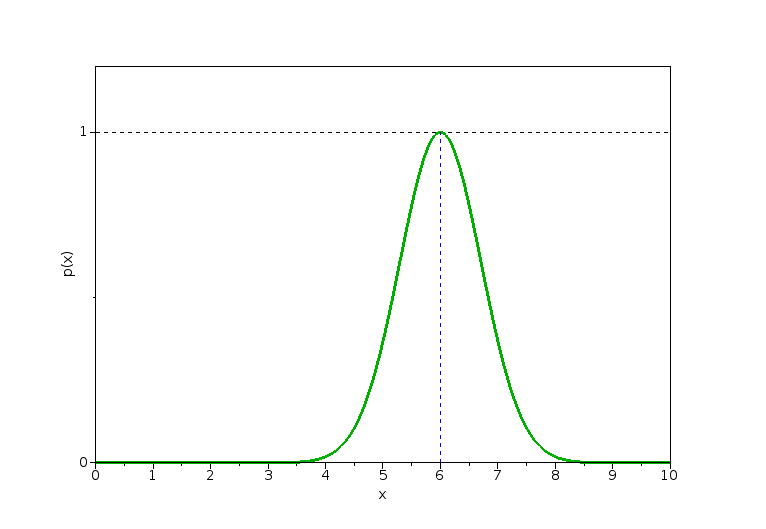
\includegraphics[width=0.85\linewidth]{./pic/fuzzy_number_intro}}
\caption{\small Функция $p(\cdot)$, заданная своим графиком на отрезке $X = [0;\,10]$ и принимающая значения на отрезке $\zo$, иллюстрирует рассматриваемый в настоящей работе вариант модели экспертной оценки. Значения её аргумента $x \in X$~--- это возможные значения оцениваемого параметра, а значния функции могут интерпретироваться, например, как степень уверенности эксперта в каждом из значений аргумента. }
\label{ris:fuzzy_number_intro}
\end{figure}

Будем считать, что эксперт выставляет оценку осознанно (не <<наобум>>) и заинтересован в достижении высокого качества экспертизы (обладает ответственностью), а потому экспертные оценки удовлетворяют условиям <<рациональности>>:
\begin{enumerate}
 \item Будучи спрошен несколько раз подряд об одном и том же, эксперт выдаст один и тот же ответ. Эксперт не является <<измерительными прибором>> с присущей последнему погрешностью измерений. 
 \item Эксперт выразит своё мнение максимально полно в рамках используемой математической модели экспертной оценки. При ответе на какой-то заданный ему вопрос, эксперт может испытывать неуверенность и высказывать её, если позволяет модель экспертной оценки.
\end{enumerate}

 Из этих условий следует, что, в отличие от модели формирования данных измерений, модель формирования экспертной оценки не является стохастической, и экспертная оценка не является случайной в теоретико-вероятностном смысле. Она не является оценкой из области математической статистики. Модель экспертной оценки, в отличие от модели данных измерений, не требует процедуры эмпирического восстановления. Сколь бы сложной она не была, она сразу и целиком задаётся экспертом, например, при ответе на поставленный ему вопрос.
  
Субъективность суждения эксперта не подразумевает запрета опираться в том числе и на объективную информацию, если она имеется в наличии в том или ином объёме. Но в математической модели неопределённости, порождаемой субъективными суждениями, мы не будем учитывать такую, в общем случае, отсутствующую информацию и будем считать, что эксперт <<извлекает>> оценку непосредственно из своего сознания. 

%Методы моделирования субъективных суждений занимают центральное место в настоящей работе. Для анализа экспертных оценок надо определить допустимые математические операции над ними и необходимые для этой цели дополнительные свойства используемых математических объектов, см. раздел \ref{sec:math_methods_global}. 

\subsection{Принятие решений}
\label{sec:intro_decision}

Слово <<решение>> в русском языке имеет несколько оттенков: 
\begin{itemize}
  \item В математике решение задачи, в зависимости от её свойств, может быть найдено аналитически или численно, подобрано случайно или не совсем случайно, получено с использованием дополнительных соображений. Решение может быть или не быть единственным, а может и не существовать вовсе,  хотя во многих случаях можно переформулировать задачу так, чтобы решение всё же существовало и было единственным хотя бы с точностью до эквивалентных решений. 
  \item В более широком смысле, в практических задачах, решение часто требуется не только найти, но и {\sl принять} (иногда --- отвергнуть). Принятие решения означает принятие человеком ответственности за его правильность. Человека, берущего на себя эту ответственность, будем называть {\sl лицом, принимающим решение}\footnote{Вообще говоря, лицом, принимающим решение, может быть как физическое, так и юридическое лицо, так и группа физических или юридических лиц.}, а действия и средства, направленные ему в помощь~--- поддержкой принятия решения. 
\end{itemize}

В настоящей работе рассматривается задача выбора объектов. Она рассматривается и как проблема, требующая принятия решения, и как математическая экстремальная задача. В контексте обычно понятно, в каком смысле используется слово <<решение>>. Если это не так, будем использовать словосочетания <<математическое решение>> и <<волевое решение>>.
 
% Решение экстремальной задачи называют оптимальным, и мы используем это слово в названии настоящей работы. Но следует помнить, что найденное оптимальное математическое решение может быть отвергнуто лицом, принимающим волевое решение.

Для поддержки принятия решений в условиях неопределённости (см. \ref{sec:intro_uncertainty}) широко применяется математическая статистика. Однако, даже в случае стохастической неопределённости её применение ограничено трудностями построения теоретико-вероятностной модели.  Например, в следующих случаях применение математической статистики затруднено:
\begin{itemize}
 \item отсутствуют фактические данные о предметах исследования за достаточно продолжительный период времени, и нет времени или принципиальной возможности их собрать; 
 \item исследуется процесс, направление развития которого нетривиальным образом зависит от событий, которые могут реализоваться или не реализоваться в будущем;
 \item исследуется качественно новое явление, процесс его развития уникален.
\end{itemize}

Важную роль для принятия решения в таких случаях неопределённости играют субъективные суждения, т.\,е. мнения компетентных людей. С развитием информационных технологий, использование субъективных суждений в практике принятия управленческих решений оказалось поставленным на математическую основу на ряду с прочими математическими методами поддержки принятия решений. В частности, широкое распространение получили экспертные оценки (см. \ref{sec:intro_subjective}).

 С этим связано появление ряда фундаментальных математических работ, посвящённых невероятностным методам моделирования неопределённости. Субъективная вероятность Сэведжа~\cite{savage1972foundations} как мера неуверенности субъекта, суждения которого удовлетворяют определённым условиям «рациональности»; верхние и нижние вероятности Демпстера~\cite{dempster}, характеризующие неполноту наблюдений и отражающие неопределённость в теории вероятностей, моделируемую многозначными отображениями; правдоподобие и доверие Шеффера~\cite{shafer}, обобщающие конструкции Демпстера в теории принятия решений; возможность Заде~\cite{citeZadeh}, основанная на его теории нечётких множеств~\cite{ZadehPrime}, — вот далеко не полный перечень таких работ. Современные работы, наследующие и обобщающие работы своих предшественников,~--- это теории возможностей Дюбуа и Прада~\cite{dubois_prade-1990, Dubois2015}, де~Кумана~\cite{de1992possibility} и Ю.~П.~Пытьева~\cite{possbook, probbook}. Из них теория возможностей Ю.~П.~Пытьева лежит в основе настоящей работы, и методы этой теории изложены в разделе \ref{sec:math_methods_ours}.  

При выставлении экспертных оценок, экспертом может быть и само лицо, принимающее решение~--- это тоже имеет смысл,~--- но чаще всего подразумевается помощь приглашённых экспертов.  Приглашённый эксперт может высказать мнение как в произвольной форме, так и в ответ на вопросы, специально сформулированные для поддержки принятия какого-либо решения. Процесс подготовки вопросов и прочих материалов, получения и последующего анализа экспертных мнений будем называть экспертным опросом или  экспертизой. Лицо, принимающее решение, или субъект, от имени которого действует это лицо, выступает здесь в роли заказчика экспертизы, а также лица, заинтересованного в результатах исследования (исследователя). От экспертов это лицо получает ответы на поставленные вопросы.

%Например, это происходит, если предметы исследования не покрываются одной конкретной предметной областью, а находятся в самых разных предметных областях. 
%\noticeheader
\begin{notice}
Если задача принятия решения в условиях неопределённости имеет научно-технический характер, то иногда её решение уже назревает в мозгу специалистов, работающих в соответствующей области. Однако, это решение может быть ещё не оформлено в виде мыслей, имеющих достаточную чёткость для выражения. Экспертный опрос, а именно, грамотно сформулированные аспекты предметов исследования и хорошие вопросы про них, помогает осознать и формализовать эти мысли, после чего на суд лица, принимающего решение, выносятся не просто экспертные мнения по изначально предложенной экспертам схеме, а готовые варианты решения. Похожие вещи происходят и в случае, когда лицо, принимающее решение~--- <<само себе эксперт>>: формализация процесса принятия решения облегчает этот процесс. 
\end{notice}

В ситуации, требующей математической поддержки принятия решения, должна быть построена математическая модель ситуации, требующей принятия волевого решения, и поставлена математическая задача поиска математического решения. Эта модель включает в себя, как составные части, модели предметов исследования вместе с выбранными параметрами, а также модели субъективных суждений экспертов (экспертных оценок).
 
%\subsection{Цель работы}
%Это пока отложим. Цель лучше вписывать в текст в самом конце работы, когда её формулировка приобретает максимальную конкретность.
%Цель настоящей работы --- исследовать новый подход к проведению экспертизы, используя высокоинформативные, но при этом математически строгие модели экспертных оценок в рамках теории возможностей Ю.~П.~Пытьева. Новый подход будет продемонстрирован на примере нескольких задач из области поддержки принятия решений с использованием экспертных оценок. Для решения этих задач на ЭВМ будет разработан демонстративный комплекс программ.
%Для решения этих задач будет раз разработать эффективные алгоритмы и комплекс программ для решения этих задач. 

